\chapter{Incremental dialogue simulation}
\label{ch:simulation}

	% In this chapter, a new simulated environment is introduced. It is based on an incremental dialogue system based on the methodology presented in Chapter \ref{ch:architecture} as well as a new incremental dialogue User Simulator (US) that is able to interact with it. The novelty of the latter is that it is able to simulate the ASR instability phenomenon.
	
	Using dialogue simulation techniques is very common in the research community \cite{Eckert1997,Pietquin2006} for several reasons like: the ability to quickly generate dialogue corpora that can be used to develop machine learning techniques, an easy way to model different populations of users and the possibility to use the same user simulator to test and compare concurrent dialogue strategies (see Chapter \ref{ch:soarl} for more details). In this chapter, a new incremental dialogue simulation framework is introduced (published is \cite{Khouzaimi2016a}). Its novelty resides in the fact that it is able to simulate the ASR instability phenomenon. First, it is presented in its most generic and abstract form that can be used by the reader to instantiate his/her own simulator that is adapted to any target domain. Then, these principles are applied in order to implement a showcase simulated environment where the service is a personal agenda manager.
	
	Later on, this simulated environment is used for two main purposes. Firstly, the slot-filling and the incremental dialogue strategies described in Chapter \ref{ch:strategies} are implemented and compared. This somehow validates the preliminary efficiency analysis led in that chapter. It also provides new analysis elements to go further and prepare a basis for the experiments with real users. Secondly, it is a very useful tool for generating data to train machine learning algorithms. In Chapter \ref{ch:rl}, it is used to train a reinforcement learning algorithm which purpose is to optimise turn-taking decisions.
						
\section{Overview}
	
	How to run dialogues with no users? The well-known answer is: by designing a User Simulator (US). Rigorously, in the case of SDSs, a US should be able to process an input audio signal and to output a new audio signal as well. Even though this method has its merits (noise and ASR imperfections are naturally taken into account), it goes against one of the main advantages of user simulation techniques which is the ability to quickly generate an important number of dialogues. Also, making an ASR module listen to a TTS and understand its message is not easy. Therefore, the user simulator elaborated here inputs and outputs text. An ASR output simulator is in charge of replicating the ASR behaviour. Figure \ref{fig:simuoverview} gives an overview of how these parts fit together in the whole architecture as well as the composition of the US. The latter is composed of five modules: The Intent Manager, the NLU, the Verbosity Manager, the NLG and the Patience Manager.
	
		\begin{figure*}[htb]
			\centering
			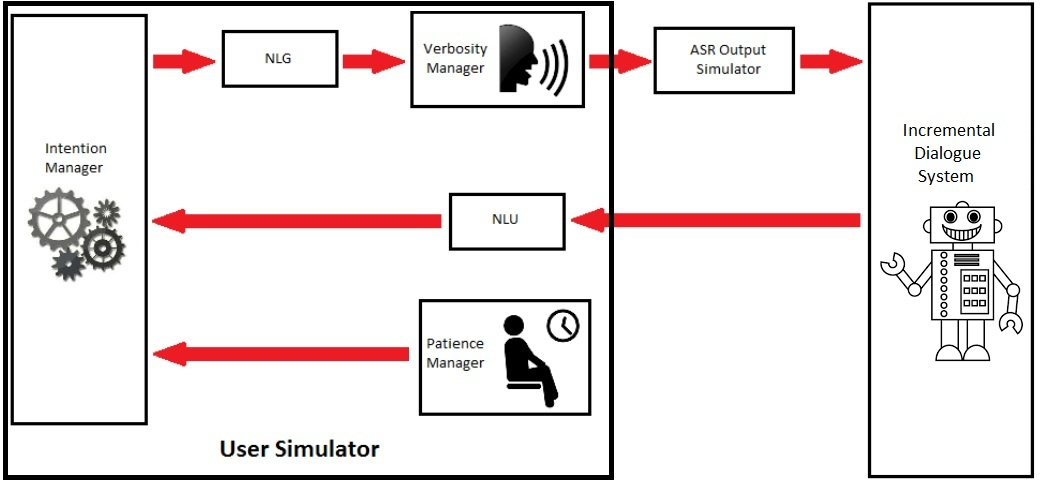
\includegraphics[scale=0.45]{figures/SimuSys.jpg}
			\caption{Simulated environment architecture}
			\label{fig:simuoverview}
		\end{figure*}
    
\section{Incremental dialogue simulation}
				
				In a nutshell, at the $p^{th}$ micro-turn of the $k^{th}$ user turn $\mu T^{k,U}_p$, the US generates a partial utterance $Req^k_p$ that is transformed into an N-Best ${(score^k_{p,1}, hyp^k_{p,1}),...,(score^k_{p,N}, hyp^k_{p,N})}$, which corresponds to the N recognition hypotheses that have the best confidence scores. It corresponds to the whole utterance pronounced during the partial turn $T^{k,U}_p$ (\textit{restart incremental} mode \cite{Schlangen2011}). On the other hand, either the US receives an answer from the dialogue system at a certain micro-turn and it stops speaking\footnote{This is of course an approximation of real barge-in cases since the overlap is neglected.}, either it does not and it continues speaking if it has additional things to say (releasing the floor otherwise). When the dialogue lasts for too long without achieving the task at hand, the US can end the dialogue.

                                In the following, the role and the functioning of the US and the ASR output simulator is discribed in an abstract fashion before being instanciated later on to give birth to a personal agenda management simulated environment.
    
	\subsection{User Simulator}

			\subsubsection{Intent Manager}
			\label{subsec:intentmanager}

					The Intent Manager is in charge of computing the dialogue acts that the US performs. It maintains an internal dialogue context and takes the dialogue acts coming from the dialogue system as inputs. Thus, it can be viewed as a dialogue manager in itself but with the difference that it is aimed to generate requests and to lead the dialogue instead of serving a user (at least in task-oriented situations). Therefore, it is given a task or a list of tasks to accomplish before it starts interacting with the dialogue system.

					A common approach to design such a module is the agenda-based method \cite{Wei1999,Schatzmann2007}. Inspired by the latter, the approach adopted in this thesis suggests that the tasks the Intent Manager should accomplish are given in the form of a stack (LIFO structure): the action stack (AS). They are removed and executed one by one and during each step, new actions could be added. The Algorithm \ref{algo:abstractim} describes a function called \textit{run} with AS as an argument and that is in charge of unstacking all the corresponding actions and executing them by using the method \textit{perform()}. The latter tries to execute the top element of the action stack which might lead to the removal of the top element of the stack or the creation of new actions that are added on top of AS (which justifies the fact that the whole stack is passed as an argument and not the top element only). A loop is run over the elements of AS until it is empty.

					\begin{algorithm}[htp]
						\DontPrintSemicolon
						\SetKwFunction{run}{run}
						\SetKwProg{myalg}{Algorithm}{}{}
						\myalg{\run{AS}}{
							\While{AS.size > 0}{
								perform(AS);
							}
						}
						\caption{Intent Manager abstract algorithm}
						\label{algo:abstractim}
					\end{algorithm}

			
			\subsubsection{NLG and Verbosity Manager}
				
				The NLG module of the simulator transforms the Intent Manager's output into a simple and straightforward utterance. For example:
				
				\begin{itemize}
					\item Book a room for tomorrow.
					\item Record channel 2 from 6pm until 8pm.
					\item Delete the event football game from the agenda.
				\end{itemize}
				
				Compared to human/human conversations, limiting interactions to this kind of simple utterances is not realistic. Therefore, they are enhanced in the Verbosity Manager with prefixes like \textit{I would like to}, \textit{Is it possible to}...and suffixes like \textit{if possible}, \textit{please}... In \cite{Ghigi2014}, a corpus study showed that users tend to go off-domain and to repeat the same information several times in the same sentence. These behaviours are also replicated in the Verbosity Manager: with a probability $p_{od}$ the NLU output is replaced with an off-domain sentence randomly picked in a predefined list, moreover, with a probability $p_{rep}$ and given that the system just reported a misunderstanding, the utterance is repeated twice (for example, \textit{Check my account, I repeat, check my account}).
			
			\subsubsection{Timing and patience manager}
			
				When it comes to incremental processing, timing is key. However, the main objective of simulation is to generate dialogues as fast as possible, hence, real time stamps cannot be used. In order to approximate durations, the user's and the system's speech rates are considered to be constant with value $SR$.
					
					Users tend to get impatient, at various degrees, when dialogue systems take too long to accomplish the task they are asked for. To simulate this behaviour, a duration threshold is chosen at each new dialogue that will cause the user to hangup as soon as it is reached. It is computed as follows
					
					\begin{eqnarray}
						d_{pat} = 2 \mu_{pat}.sigmoid(X)
					\end{eqnarray}
					
					where X follows a Gaussian distribution of mean 0 and variance 1 and $\mu_{pat}$ is the mean duration since
					
					\begin{eqnarray}
						sigmoid(x) & = & \frac{1}{1 + e^{-x}}
					\end{eqnarray}
					
					
	\subsection{ASR output simulator}
			
				The ASR output simulator generates an N-Best that is updated at each new micro-turn. For instance, if at a certain point, the US uttered \textit{I would like to add the event birthday party on...}, a possible N-Best could be (the numbers between brackets represent ASR scores):
					
					\begin{itemize}
						\item (0.82) I would like to add the event birthday party on
						\item (0.65) I like to add the event birthday party on
						\item (0.43) I have had the event birthday party
						\item (0.33) I would like to add the holiday party
						\item (0.31) I like to add the holiday party on
					\end{itemize}
					
					More formally, at the $p^{th}$ micro-turn of the $k^{th}$ user turn $\mu T^{k,U}_p$, the N-Best is an N-uplet ${(score^k_{p,1}, hyp^k_{p,1}),...,(score^k_{p,N}, hyp^k_{p,N})}$. At time t+1, a new word $w_{t+1}$ is sent to the ASR output simulator and the latter calculates a new associated N-Best. Therefore, at this stage, the system has two N-Bests:
					
					\begin{itemize}
						\item \textbf{The word N-Best:} It corresponds to the different hypotheses related to the last word pronounced. In Figure \ref{fig:asrsimu}, the top right box represents the word N-Best associated with the word $6^{th}$.
						\item \textbf{The utterance N-Best:} It designates the N-Best associated with the whole partial utterance pronounced so far. In Figure \ref{fig:asrsimu}, the top left box is an a example of such N-Best associated with the partial utterance \textit{I want to add the event birthday party on January}.
					\end{itemize}
					
					Both are combined to form the new utterance N-Best. In the following, the way the word N-Best is calculated and the way it is incorporated into the partial utterance N-Best are described.
					
					In order to simulate noise and ASR imperfections, the ASR output simulator uses a module called the Scrambler. It receives a word as input and performs one of the three following operations in order to compute the output\footnote{The Scrambler always performs one these three operations. In other words $p_{repl} + p_{add} + p_{del} = 1$}:
					
					\begin{itemize}
						\item Replace the word with a different word taken randomly from a dictionary (probability: $p_{repl}$)
						\item Add a new word (probability : $p_{add}$)
						\item Delete the word (probability : $p_{del}$)
					\end{itemize}
					
					A Word Error Rate (WER) is given as a parameter to the ASR output simulator. It controls the noise level that one wants to simulate. The algorithm used to generate the N-Best associated with a single word is described below:
					
					\begin{figure}[t]
					\centering
					\begin{tikzpicture}[scale=0.8]
					\begin{axis}[
						xlabel={Confidence score},
						ylabel={Density},
						scaled ticks = false,
						tick label style={/pgf/number format/fixed},
						xmin=0, xmax=1,
						ymin=0, ymax=0.55,
						xtick={0,0.2,0.4,0.6,0.8,1},
						ytick={0.1,0.2,0.3,0.4,0.5,0.6},
											legend pos=north east,
						ymajorgrids=true,
						grid style=dashed,
											colorbrewer cycle list=Set2,
					]
					
					\addplot+[
						error bars/.cd,
						y dir=both,
						y explicit,
						]
						coordinates {
						(0,0)
	(0.1,0.19483312081792062)
	(0.2,0.3702598583755481)
	(0.3,0.3943180330023535)
	(0.4,0.33431406881442405)
	(0.5,0.24197072451914337)
	(0.6,0.1485840305841884)
	(0.7,0.07242576116369753)
	(0.8,0.023141241148471745)
	(0.9,0.00240534717059161)
	(1,0)
						};
											
											\addplot+[
						error bars/.cd,
						y dir=both,
						y explicit,
						]
						coordinates {
						(0,0)
	(0.1,0.002405347170591614)
	(0.2,0.023141241148471745)
	(0.3,0.0724257611636976)
	(0.4,0.14858403058418854)
	(0.5,0.24197072451914337)
	(0.6,0.33431406881442416)
	(0.7,0.3943180330023536)
	(0.8,0.37025985837554803)
	(0.9,0.1948331208179205)
	(1,0)

						};
											

					\legend{Bad recognition,Good recognition}

					\end{axis}
					\end{tikzpicture}
					\caption{ASR score sampling distribution ($\sigma_{conf} = 1$)}
					\label{fig:scoresample}
			\end{figure}
			
					\begin{enumerate}
						\item Determine whether $w_{t+1}$ is among the N-Best or not with a probability that is computed as follows: (1 - WER) + INBF.WER, where INBF (In N-Best Factor) is a parameter between 0 and 1. If $w_{t+1}$ is not in the N-Best, then the latter contains only scrambled versions of this word and jump to step 4.
							\item The first hypothesis is set to be $w_{t+1}$ with a probability of (1-WER), otherwise, it is a scrambled version of it.
							\item If the the first hypothesis is not $w_{t+1}$, then this word's position is randomly chosen between 2 and N. Moreover, the other hypotheses are scrambled versions of it.
							\item The confidence score associated with the best hypothesis ($score_0$) is sampled as sigmoid(X) where X follows a Gaussian distribution. More precisely,\\$X \sim \mathcal{N} (c_{err},\sigma_{conf})$ if the first hypothesis is wrong and $X \sim \mathcal{N} (c_{right},\sigma_{conf})$ when it is right (with $c_{err} < 0 < c_{right}$). By taking the sigmoid, this leads to two distributions\footnote{Confidence score estimation is a complex problem and it is still a research topic \cite{Jiang2005,Seigel2011}. The simple model introduced here is inspired by \cite{Pietquin2005}. Also, notice that the scores are between 0 and 1 but they do not sum up to 1 since they are not probabilities.} (depicted in Figure \ref{fig:scoresample} for $\sigma_{conf} = 1$) with a mean on both sides of 0.5 and the same standard deviation for both (which is a growing function of $\sigma_{conf}$ and which can be changed to simulate different levels of accuracy of the confidence score model). Big $\sigma_{conf}$ values lead to spread recognition scores and small differences between $c_{err}$ and $c_{right}$ engender close scores for both cases: right and wrong first hypothesis. Therefore, discriminative models are obtained for small values of $\sigma_{conf}$ and high difference $c_{right}-c_{err}$.
							\item The scores for the other hypotheses are computed in an iterative way. For $i$ between 2 and N, $score_i$ is uniformly sampled in $[0,score_{i-1}]$.
					\end{enumerate}
					
					As already mentioned in this thesis, early partial utterances are not necessarily prefixes of later ones with a true ASR system (ASR instability phenomenon). To replicate this behaviour, a language model is needed to compute the scores corresponding to the different hypotheses in the N-Best. Therefore, sentences that are more in alignment with the model have higher scores thus being pushed to the top of this N-Best. Here, the NLU knowledge is used as a proxy for the language model by making the following assumption: \textit{the more an utterance generates key concepts once fed to the NLU, the more it is likely to be the correct one}. Therefore, as soon as a new concept is detected in $hyp^k_{p,i}$, $score^k_{p,i}$ is boosted as follows:
					
						$$ score^k_{p,i} \leftarrow score^k_{p,i} + BF.(1 - score^k_{p,i}) $$
							
					where BF is the Boost Factor parameter. An illustration of this mechanism with BF=0.2 is provided in Fig. \ref{fig:asrsimu}.
					
					\begin{figure*}[h]
						\centering
						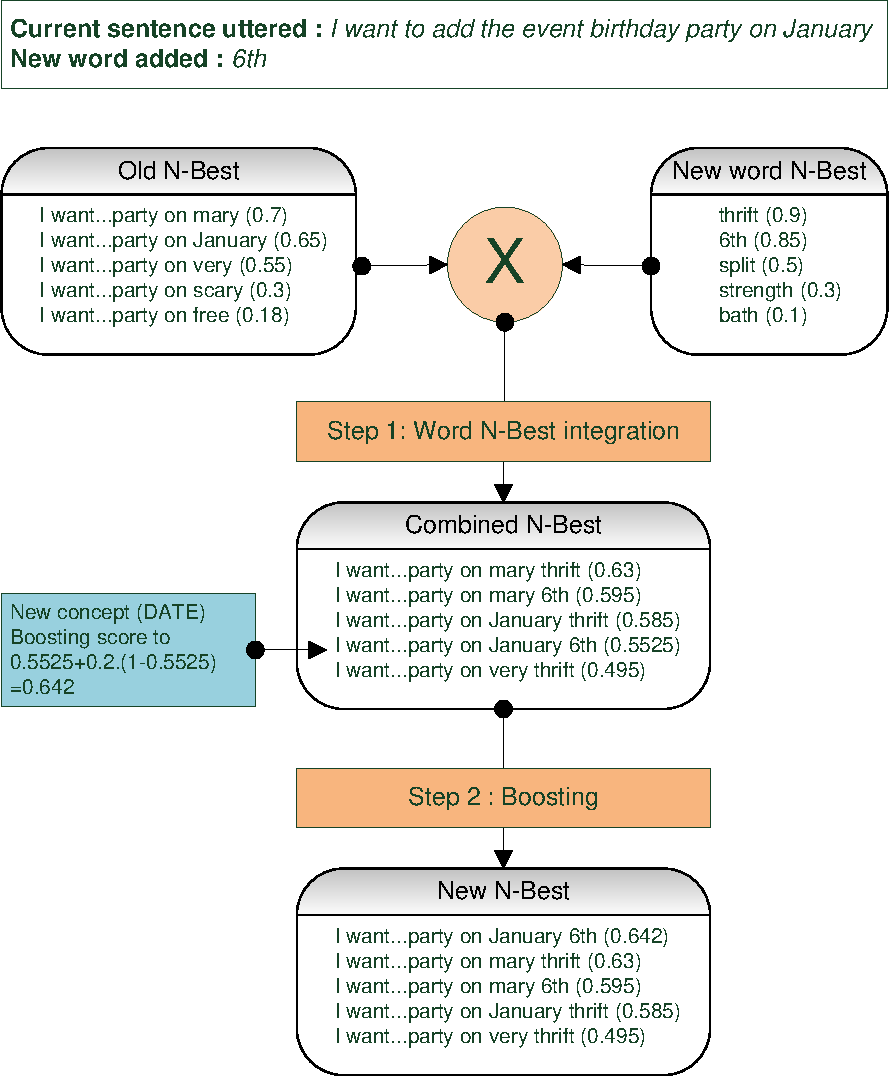
\includegraphics[scale=0.75]{figures/ASRSimu.pdf}
						\caption{An illustration of the incremental ASR output N-Best update (BF=0.2)}
						\label{fig:asrsimu}
					\end{figure*}

\section{Personal Agenda management simulated environment}

	So far, an abstract framework for simulating incremental dialogues has been described. In this section, it is instanciated to be able to generate dialogues with an incremental dialogue system which purpose is to help users manage their personal agenda. This task will be used in Chapter \ref{ch:baseline} in order to run a few experiments regarding the dialogue strategies introduced in Chapter \ref{ch:strategies} and in Chapter \ref{ch:rl} to test a new reinforcement learning approach. First the Service (system side, Section \ref{subsec:service}) and its dialogue task are presented, then the way the US (user side, Section \ref{subsec:us}) and the ASR output simulator are instanciated is described.
	
	\subsection{The Service: personal agenda assistant}
        \label{subsec:service}
	
		\subsubsection{Dialogue Manager}

			A personal agenda assistant has been implemented as a new task for the experiments. The user can add, move or delete events in his agenda. For instance, a request could be: \textit{I would like to add the event football game on March $3^{rd}$ from 9 to 10 pm}\footnote{The dialogues are actually in French but they are translated in English to ensure language coherence in this thesis.}. This is a slot-filling task with four slots:
				
				\begin{itemize}
					\item \textbf{ACTION:} The type of action the user wants to perform. Can take three different values: ADD, MODIFY or DELETE.
						\item \textbf{DESCRIPTION:} The description of the event.
						\item \textbf{DATE:} The date of the event.
						\item \textbf{WINDOW:} The time window of the event.
				\end{itemize}
				
				However, no overlap is tolerated between events in the agenda.
				
				Each interaction between the US and the system is defined by a scenario. Here, the US is given two lists of events: \textit{InitList} and \textit{ToAddList}. The first one contains the events that already exist in the agenda before the dialogue and the second one contains the ones that the US is supposed to add during the dialogue. Each event is associated with a priority value and the US must prefer adding the ones with high priority first\footnote{To make the algorithms easier to understand, the larger priority value, the more important the event, unlike common usage.}. Its aim is to make as many events with the highest priority values as possible fit in the agenda.
				
		
		\subsubsection{Natural Language Understanding}
		
			A rule-based algorithm transforms the user's utterance hypothesis into concepts. To do that, a set of rules have been defined. Each rule transforms a word, a concept or any combination of the two into a new concept. Three types of rules are used; they are depicted in Table \ref{tab:ruletypes}.
			
			For instance, parsing the sentence \textit{I want to add the event birthday party on January $6^{th}$ from 9pm to 11pm} is performed following these steps:
							
							\begin{enumerate}
						\item \textbf{I want to ADD the TAG\_EVENT birthday party on MONTH(January) NUMBER(6) from TIME(9,0) to TIME(11,0)}
								\begin{itemize}
										\item add : [ADD]
											\item event : [TAG\_EVENT]
											\item Regex(janvier|...|decembre) : MONTH(\$word)
											\item Regex([0-9]+) : NUMBER(\$word)
											\item Regex((([0-1]?[0-9])|(2[0-3]))h([0-5][0-9])?) : TIME(\$word)\footnote{Adapted to the french way of uttering time values.}
									\end{itemize}
							\item \textbf{I want to ADD the TAG\_EVENT birthday party on DATE(6,1) \\ WINDOW(TIME(21,0),TIME(23,0))}
								\begin{itemize}
										\item Combine(NUMBER,MONTH) : DATE(NUMBER,MONTH)
											\item Combine(from,TIME\_1,to,TIME\_2) : WINDOW(TIME\_1,TIME\_2)
									\end{itemize}
							\item \textbf{I want to ADD EVENT(birthday party, DATE(6,1), \\ WINDOW(TIME(21,0),TIME(23,0)))}
								\begin{itemize}
										\item Combine(TAG\_EVENT,\$x,on,DATE,WINDOW) : EVENT(\$x,DATE,WINDOW)
									\end{itemize}
							\item \textbf{I want ACTION(ADD, EVENT(birthday party, DATE(6,1), \\ WINDOW(TIME(21,0),TIME(23,0))))}
								\begin{itemize}
										\item Combine(ADD,EVENT) : ACTION(ADD,EVENT)
									\end{itemize}
					\end{enumerate}
					
			\subsection{Simulator instanciation}
                        \label{subsec:us}
			
				\begin{table}[t]
					\fontsize{8}{10}\selectfont
					\vspace{2mm}
					\centerline{
						\begin{tabular}{|l|l|l|}
							\hline
							\textbf{Rule type} & \textbf{Description} & \textbf{Example} \\
							\hline
							Tag & Words are associated with labels & remove : [DELETE] \\
							Regular expressions & Words matching a regular expression & Regex([0-9]+) : NUMBER(\$word) \\
							& are transformed into concepts & \\
							Combine & Words and concepts are mapped into a new concept & Combine(NUMBER,MONTH) : DATE \\
							\hline
						\end{tabular}
					}
					\caption{\label{tab:ruletypes} {NLU rules types}}
				\end{table}
			
				\begin{algorithm}[htp]
					\DontPrintSemicolon
					\SetKwRepeat{Do}{do}{while}
					\SetKwFunction{run}{run}
					\SetKwProg{myalg}{Algorithm}{}{}
					\myalg{\run{AS}}{
						\While{AS.size > 0}{
							altQ $\gets$ AS.top.event.alt\;
							c $\gets$ empty map\;
							M $\gets$ empty map\;
							\Do{altQ.size > 0 AND conflQ.size > 0}{
								conflQ $\gets$ execute((AS.top.action,altQ.next))\;
								\If{conflQ.size > 0}{
									c.add(altQ.next,conflQ)\;
									M.add(altQ.next,$\max_{e \in \text{conflQ}}$ e.prio)\;
									altQ.removeNext()\;
								}
							}
							\eIf{conflQ.size > 0}{
								$e_{best} \gets$ argmin(M)\;
								\eIf{M($e_{best}$) < AS.top.event.prio}{
									\For{e $\in$ c($e_{best}$)}{
										\eIf{e.alt.size > 1}{
											\For{e' $\in$ e.alt-\{e\}}{
												AS.add((MOVE,e'))\;
											}
										}{
											AS.add((DELETE,e))\;
										}
									}
								}{
									AS.removeTop()\;
									\If{AS.top.action == MOVE}{
										AS.add((DELETE,AS.top.event))\;
									}
								}
							}{
								AS.removeTop()\;
							}
						}
					}{}
					\caption{Intent Manager algorithm}
					\label{algo:intent}
				\end{algorithm}
			
				\begin{table}[htp]
						\fontsize{8}{10}\selectfont
						\vspace{2mm}
						\centerline{
							\begin{tabular}{|l|l|l|}
								\hline
								\textbf{Parameters} & \textbf{Value} & \textbf{Justification} \\
								\hline
								$p_{od}$ & 0.1 & Based on the corpus study led in \cite{Ghigi2014} \\
								$p_{rep}$ & 0.3 & Id. \\
								$SR$ & 200 words per minute & See \cite{Yuan2006} \\
								$\mu_{pat}$ & 3 min & Empirical given the task \\
								$p_{repl}$ & 0.7 & Empirical (variable and difficult to estimate) \\
								$p_{add}$ & 0.15 & Id. \\
								$p_{del}$ & 0.15 & Id. \\
								N & 5 & Empirical (can be anything depending on the ASR configuration) \\
								INBF & 0.7 & Tuned for a reasonable boosting effect with N=5 \\
								BF & 0.2 & Id. \\
								$c_{err}$ & -1 & Empirical (variable and difficult to estimate) \\
								$c_{right}$ & 1 & Empirical (variable and difficult to estimate) \\
								$\sigma_{conf}$ & 1 & Id. \\
								SM & 2 & words that lasted for more than 0.6 seconds have 90\% chance \\
								& & of staying unchanged \cite{McGraw2012} \\
								& & and SR = 200 wpm \\
								WER & Variable during the experiments & \\
								\hline
							\end{tabular}
						}
						\caption{User simulator and ASR output simulator values}
						\label{tab:paramvalues}
					\end{table}
			
				The aim of the US is to make the biggest number possible of events with the highest priority values taken from \textit{InitList} and \textit{ToAddList} fit in the agenda. To do so, the Intent Manager executes the \texttt{run()} function (taking the action stack (\texttt{AS}) as an argument) depicted in Algorithm \ref{algo:intent} (an instance of the abstract function depicted in Algorithm \ref{algo:abstractim}) where
				
				\begin{itemize}
					\item The manipulated structures are stacks and queues.
					\item If \texttt{st} is a stack, the top element is called \texttt{st.top} and \texttt{st.removeTop()} removes it from \texttt{st}.
					\item If \texttt{q} is a queue, the next element is called \texttt{q.next} and \texttt{q.removeNext()} removes it from \texttt{q}.
					\item The size of the structure \texttt{x} is called \texttt{x.size}.
					\item If \texttt{m} is a map, \texttt{m.add(x,y)} adds a new entry to m such that \texttt{m(x) = y}.
					\item \texttt{AS} is a stack of actions and each action a is a couple (\texttt{a.action},\texttt{a.event}) where \texttt{a.action} is an action type (ADD, MODIFY or DELETE) and \texttt{a.event} is an event caracterised by a description, a date, a time window and a priority value.
					\item For each event \texttt{e}, \texttt{e.alt} refers to all its alternatives including itself\footnote{The elements of \texttt{e.alt} share the same description and priority value but they have different dates and time windows.}. Its priority is called \texttt{e.prio}.
					\item The function \texttt{execute()} communicates an intent to the NLG and gets the corresponding response through the NLU. If this response is a misunderstanding declaration, then the same intent is sent again. If it is a declaration of conflict with a set of other events, then a queue with all these events is returned. Finally, if no conflict was detected, then this function returns an empty queue. This is how the US updates \texttt{AS}.
				\end{itemize}
						
					The other parameters of the US and the ASR output simulator are set as shown in Table \ref{tab:paramvalues}.
					
\section{Functionning illustration}
			
				The following illustration provides the reader with a global view of all the notions introduced in this chapter through an application to a concrete interaction in the agenda management domain. Consider the following scenario:
				
				\begin{itemize}
					\item \textbf{InitList:} \{\textbf{title:} \textit{house cleaning}, \textbf{date:} \textit{January $6^{th}$}, \textbf{window:} \textit{from 18 to 20}, \textbf{priority:} \textit{3}, \textbf{alternative 1:} \textit{January $7^{th}$, from 6pm until 8pm}, \textbf{alternative 2:} \textit{January $9^{th}$, from 10am until 12am}\}
					\item \textbf{ToAddList:} \{\textbf{title:} \textit{birthday party}, \textbf{date:} \textit{January $6^{th}$}, \textbf{window:} \textit{from 6pm until 11pm}, \textbf{priority:} \textit{5}\}
				\end{itemize}
				
				\texttt{AS} initially contains the ADD action associated with the event \textit{birthday party} since it is the only event in \textit{ToAddList}. Let \texttt{e} be this event. The function \texttt{run()} in Algorithm \ref{algo:intent} is then run over this stack. Thus the first result generated by the Intent Manager is the ADD action corresponding to the event \textit{birthday party}. Once communicated to the NLG, the latter outputs the sentence \textit{Add the event birthday party on January $6^{th}$ from 6pm until 8pm} which is in turn transfered to the Verbosity Manager. $p_{od}=0.1$ so there is a 10\% chance that the result of the NLG is ignored and replaced by an off-domain sentence. Suppose it is the case for this first trial then the ASR output simulator's result is also off-domain. As a consequence, the service responds by saying that the user's requests has not been understood which is recognised as a dialogue act by the NLU and communicated to the Intent Manager. The function \texttt{execute()} then sends the same intent once again to the NLG which generates the same utterance as it did the first time. As the last system's response is a misunderstanding declaration, the Verbosity Manager has $p_{rep}=0.3$ chance of repeating the same sentence twice. Suppose it is the case, then the Verbosity Manager's output is the following (a prefix and a suffix are also randomly added by this module): \textit{Can you please add the event birthday party on January $6^{th}$ from 6pm until 8pm, I repeat, add the event birthday party on January $6^{th}$ from 6pm until 8pm if it is possible}. The ASR output simulator generates an N-Best as it is described in Figure \ref{fig:asrsimu}.
				
				Suppose that \textit{CommitCond} in the Scheduler is true if and only if the response to the last stable utterance is either a confirmation question or a conflict declaration (in other words, all the slots have been successfully communicated to the system). Also, suppose that this time, the best ASR hypothesis is 100\% correct. Since SM=2, the Scheduler decides to take the floor as soon as the users decides to utter \textit{Can you please add the event birthday party on January $6^{th}$ from 6pm until 8pm, I repeat}.
				
				Since the time window required to organise the birthday party is already taken by the house cleaning event \texttt{execute()} returns a queue (\texttt{conflQ}) containing the latter only, and the entry (\texttt{e},\texttt{conflQ}) is added to \texttt{c}. The priority of the house cleaning event is 3, therefore, the entry \texttt{(e,3)} is added to \texttt{M}. Therefore, $e_{best} =$ \texttt{e} since it is the only element in \texttt{M}. Its priority is lower than \texttt{AS.top.event.prio}. As a consequence, the Intent Manager tries to move the house cleaning event (details about the sentence formulation and management are no longer given) and it ends up to be successful using the first alternative: \textit{January $7^{th}$, from 6pm until 8pm}. By doing so, the event \textit{birthday party} is still in the stack and it is added facing no problem this time since the corresponding time window has been freed.

                                To sum up, a new incremental dialogue simulation which supports dialogue instability has been introduced in detail in this chapter. Its different components have been thoroughly described as well as the way they interact with each other to incrementally send requests to the system and to process its responses. In the rest of this thesis, the strategies formerly described are implemented and evaluated in this simulated environment, then the latter is used to train a reinforcement learning turn-taking strategy.
